\section{USB-C Output Stage}
\label{sec:hw-usbc}

The MPQ4242GVE-0000-AEC1-P stage regulates the USB-C output voltage from the isolated bulk supply. The stage includes the switching inductor, output power path, current-sense element, bulk and ceramic capacitors, CC connections, data-line protection, and VBUS TVS protection. In \Cref{fig:schematic-usbc}, \texttt{V\_PW\_OUTPUT\_BULK} feeds the stage and \texttt{USB\_PD\_OUT} supplies the USB-C output.

\begin{landscape}
\begin{figure}[htbp]
\centering
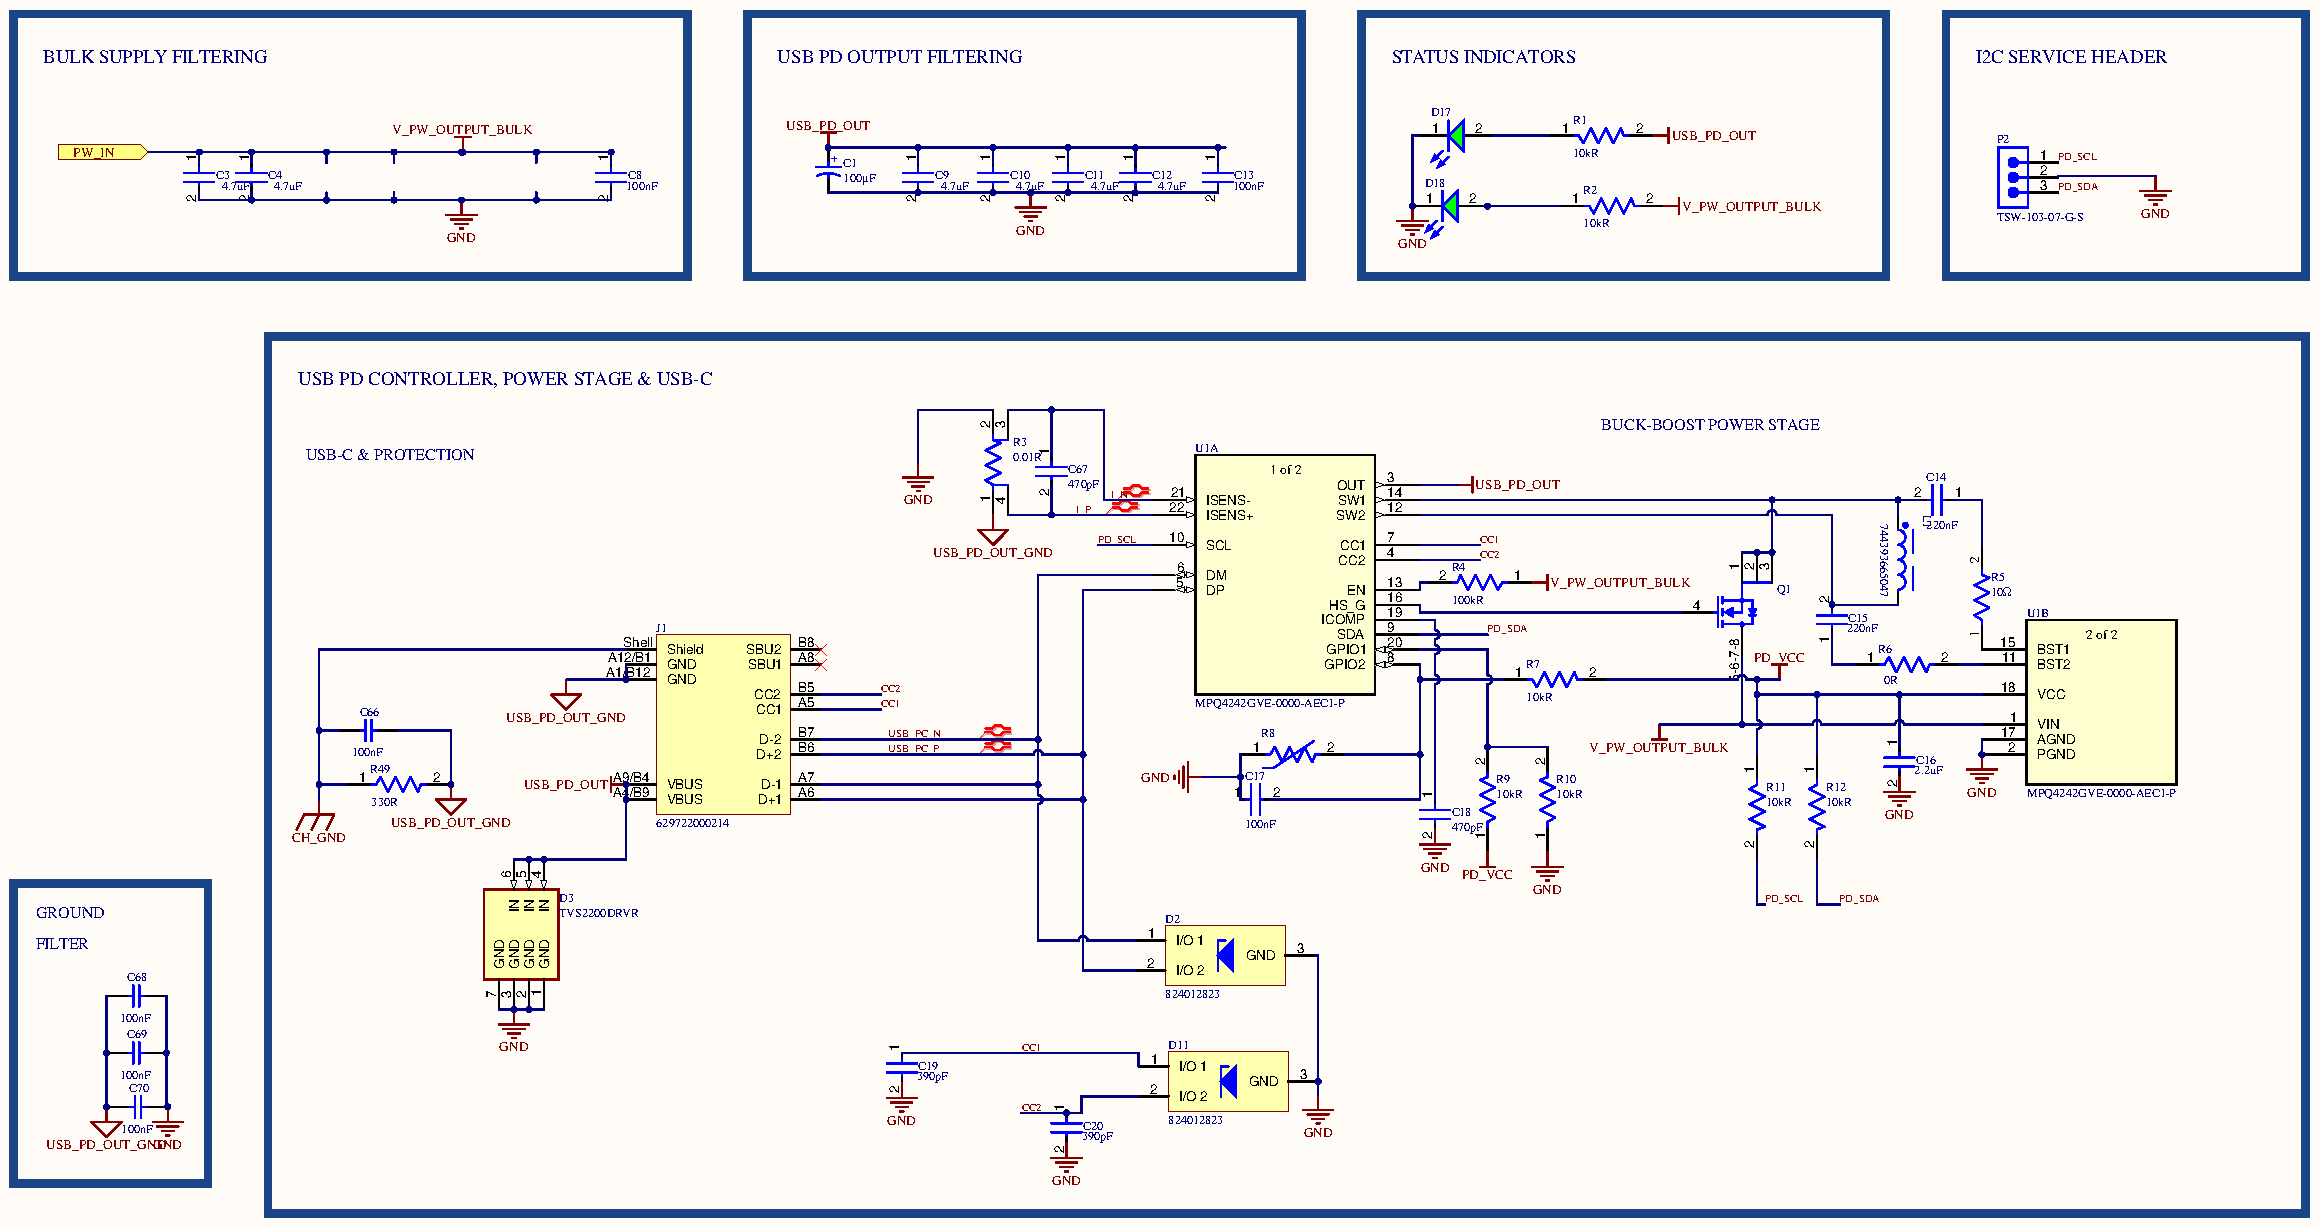
\includegraphics[width=0.97\linewidth,height=0.76\textheight,keepaspectratio]{Pictures/Thesis/07_Hardware/Rebuilt/schematic_v2_usb_excerpt.pdf}
\caption{V2 sheet 2: MPQ4242 output stage, USB-C connector, current sensing, capacitors, and interface protection.}
\label{fig:schematic-usbc}
\end{figure}
\end{landscape}

The \SI{5}{\volt}, \SI{9}{\volt}, \SI{15}{\volt}, and \SI{20}{\volt} fixed outputs were tested. According to the project notes, the \SI{20}{\volt} setting is advertised for up to \SI{5}{\ampere}. A \SI{100}{\watt} operating point was not reached in the completed tests.

The MCU regulates the secondary bulk voltage using feedback at PA1. The USB-C PD stage regulates its output to the selected PD level. Voltage at the load can differ because of cable drop, so the measurement point is stated with each result. The fixed-output tests confirmed operation of the assembled path at those settings. USB-PD negotiation and interoperability still need protocol testing.
